\scanpage{125}
semi-simples, \deleted{,}on a une catégorie qui n'est plus graduée, seulement filtrée, \deleted{I} Si $V$ est la catégorie des schémas de type fini sur un corps fixé, $M$ la catégorie des motifs sur ce même corps (\deleted{a}p\deleted{v}résumée avec toutes les données et conditions de 1\textsuperscript{\uline{o}}\deleted{)}\handwritten{)}\handwritten{\unsure{\deleted{t}|4|\deleted{(}}}, on doit avoir un foncteur \deleted{\unsure{$V$|$Y$}} compatible avec ces structures \deleted{de} (cohomologie motivique)
\[
h:V\handwritten{\longrightarrow}\unsure{\deleted{\mathrm E}G|\deleted{C}G|G|E}\mathrm{ra}\deleted{,}\mathrm{d}(M)\handwritten{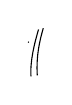
\begin{tikzpicture}[x=.4cm,y=.4cm,baseline=-.2ex]\draw (.08,-.75) .. controls (.04,-.20) and (.25,.50) .. (.32,.74);\draw (.28,-.72) .. controls (.24,-.10) and (.36,.40) .. (.47,.78);\fill (0,.34) circle (.025);\end{tikzpicture}}\quad\text{(structure de Koko sur }\mathrm{Grad}(M)\text{)}\handwritten{,}
\]
et on désire que les foncteurs cohomologiques habituels sur $V$ se factori\unsure{s\deleted{e}ant|s\deleted{n}ant|s\deleted{r}ant} par \deleted{$M$. Ceci impose}\inserted{des foncteurs sur $M$. On voudra\handwritten{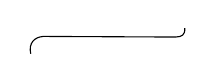
\begin{tikzpicture}[x=.4cm,y=.4cm,baseline=-.2ex]\draw (0,-.35) .. controls (-.08,.0) and (.13,.18) .. (.40,.20)--(4.6,.18) .. controls (4.80,.19) and (4.90,.24) .. (4.89,.46);\end{tikzpicture}}} que les foncteurs \deleted{fibres} obtenus sur $M$ so\deleted{n}i\unsure{\deleted{\unsure{t|n}}e|\deleted{e}\deleted{t}n}\deleted{t}nt des foncteurs fibres \deleted{\uline{tordus} seulement} véritables\inserted{\handwritten{(non tordus)}\handwritten{\begin{tikzpicture}[x=.4cm,y=.4cm,baseline=-.2ex]\draw (0,-.40) .. controls (.18,-.12) and (.28,.02) .. (.54,.07)--(2.70,.38) .. controls (2.86,.40) and (2.99,.45) .. (2.96,.63);\end{tikzpicture}}}, ce qui n'est pas idiot, \deleted{car}\inserted{\handwritten{\unsure{Car|car}}} on avait mis la structure de symétrie de Koko sur $\mathrm{Grad}(M)$: on s'est débarassé ainsi une fois pour toutes de la ``torsion''.

On peut aussi, pour parler de vrais foncteurs fibres sur la catégorie des motifs semi-simples, remplacer la donnée de symmétrie ``géométrique'' i.e. de Koko pour le produit tensoriel dans \deleted{$\mathrm{Grad}(M)$}\inserted{la catégorie graduée $M$\handwritten{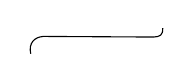
\begin{tikzpicture}[x=.4cm,y=.4cm,baseline=-.2ex]\draw (0,-.35) .. controls (-.08,.0) and (.13,.18) .. (.40,.20)--(3.9,.18) .. controls (4.10,.19) and (4.20,.24) .. (4.19,.46);\end{tikzpicture}}}, par la même canulée par le signe $(-1)^{ij}$ quand on a des \deleted{\unsure{r|e}}a\deleted{a}rguments de degré $i,j$.

11) Bien sûr, il y a lieu de chercher des théorèmes de structure intrinsèques, en termes de gerbes, pour des catégories $\unsure{\deleted{\mathrm N}C|\deleted{V}C|\handwritten{\mathfrak{C}}|\handwritten{\mathscr{C}}|\mathbb{C}}$ munies des structures de 1\textsuperscript{\uline{o}},\inserted{avec $k=\mathrm{End}(\underline{1})$ un corps donné.\handwritten{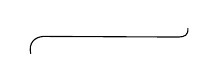
\begin{tikzpicture}[x=.4cm,y=.4cm,baseline=-.2ex]\draw (0,-.35) .. controls (-.08,.0) and (.13,.18) .. (.40,.20)--(4.7,.18) .. controls (4.90,.19) and (5.00,.24) .. (4.99,.46);\end{tikzpicture}}} Il y a lieu au besoin de supposer qu'il existe une extension de $k$ sur laquelle il y ait un foncteur fibre t\deleted{r}o\deleted{o}rdu gradué (ou m\unsure{\deleted{u}l|\deleted{l}u|\deleted{b}l|b}tigradué ? Mais où s'arrêter ? ). Le plus beau serait évidemment de trouver un théorème de structure g\deleted{g}énéral, sans \uline{supposer} l'existence d'un foncteur fibre plus ou moins tordu où que ce soit, en définissant une notion assez générale de foncteur fibre tordu (?) et en \unsure{p|\deleted{r}p}\unsure{\deleted{p}r|\deleted{r}p}\unsure{\deleted{u}o|o}uv\deleted{q}ant qu'i\deleted{p}l y en a toujours sur une extension convenable de $k$.
